\documentclass[
	english,%globale Übergabe der Hauptsprache
%	logofile=example-image-duck, %Falls die Logo Dateien nicht vorliegen
	authorontitle=true,
	]{bfhbeamer}


\usepackage[main=english]{babel}
\usepackage{tikz}  
\usepackage{tikzsymbols}
\usepackage{tikzducks}
\usepackage{amsmath}
\usepackage{caption}

% Der folgende Block ist nur bei pdfTeX auf Versionen vor April 2018 notwendig
\usepackage{iftex}
\ifPDFTeX
\usepackage[utf8]{inputenc}%kompatibilität mit TeX Versionen vor April 2018
\fi


%Makros für Formatierungen der Doku
%Im Allgemeinen nicht notwendig!
\let\code\texttt

\title{Bachelor Thesis}
\subtitle{Unlinkability of Verifiable Credentials in a practical approach}
\author[J. Robles]{Joel Robles}
\institute{TI}
\titlegraphic*{\includegraphics{example-image-duck}}%is only used with BFH-graphic and BFH-fullgraphic
\date{April 23, 2024}

%Activate the output of a frame number:
% \setbeamertemplate{page number in foot}[framenumber]


\AtBeginSection{\sectionpage}

\begin{document}

\maketitle

\begin{frame}{Table of Contents}
    \tableofcontents
\end{frame}

\section{Goal}

\begin{frame}{What is the goal?}
    The goal is to analyze the BBS Signature Scheme in conjunction with VCs in concrete use-cases and to ascertain that there is no linkability or data-leakage for real-world implementations.
\end{frame}

\section{Self-sovereign Identity}

\begin{frame}{What is Self-sovereign Identity (SSI)?}
    \begin{itemize}
        \item Is a concept, where a Person, also known as holder, can decide who gets to know what about them
        \item The state at the moment, holder has no control over their data
        \item They are not able to choose what data is shared and what not, also known as selective disclosure
        \item For example, if we show our government ID, which is a set of data or also known as a set of attributes, the verifier sees all the information on there
        \item Other problem, if a holder shows his data to someone who wants to verify it, also known as verifier, and then shows the same data to a second verifier, they can be linked
    \end{itemize}
\end{frame}

\begin{frame}{Trust Triangle}
    \begin{columns}[onlytextwidth,T]
        \column{70mm}  
        
        \begin{itemize}
            \item But how does the verifier know that the set of attributes, which is also known as a credential, is valid?
            \item He trusts the issuer!
            \item Example: Swiss government ID has holograms
        \end{itemize}

        \column{70mm}

        \begin{figure}
            \centering
            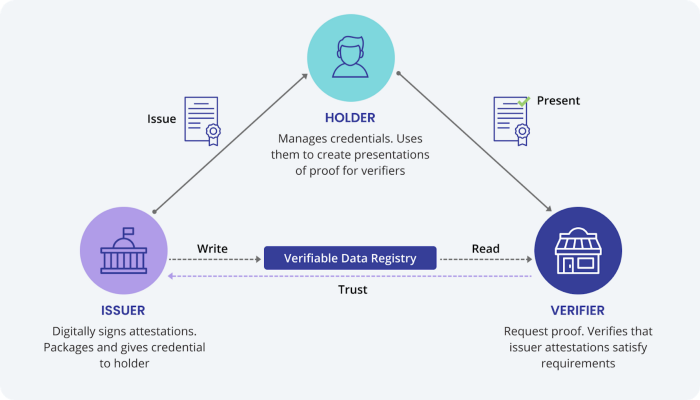
\includegraphics[width=70mm]{./img/trusttriangle.png}
            \caption{Trust triangle}
        \end{figure}
        
    \end{columns}
\end{frame}

\section{Verifiable Credentials}

\begin{frame}{Verifiable Credentials (VC)}
    \begin{columns}[onlytextwidth,T]
        \column{70mm}  

    \begin{itemize}
        \item Now we would like to recreate these physical credentials digitally
        \item We chose Verifiable credentials to represent the physical credentials digitally
        \item These are JSON-LD Objects that represent attributes in as key-value pairs
        \item Example: The first name on the government ID, is represented as \{"first\_name": "Joel"\}, where "first\_name" is the key and "Joel" is the value
    \end{itemize}

    \column{70mm}
    \begin{figure}
        \centering
        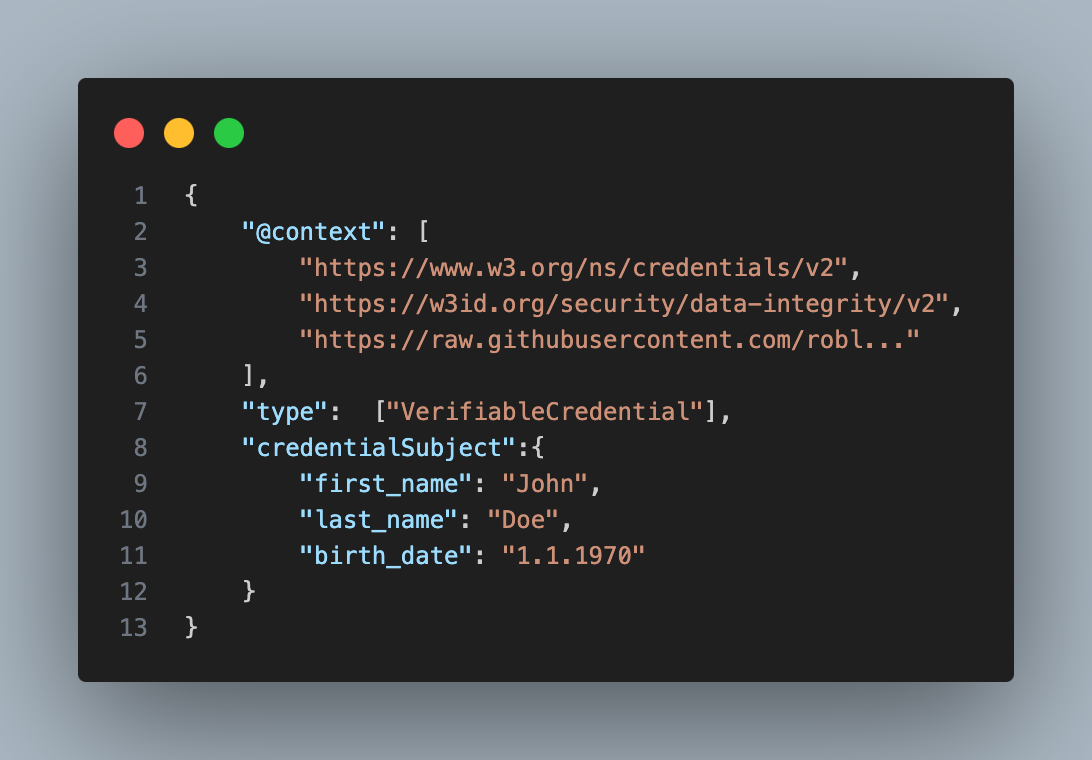
\includegraphics[width=70mm]{./img/VCexp.png}
        \caption{Example VC}
    \end{figure}

    \end{columns}
\end{frame}

\begin{frame}{VCs and BBS}
    \begin{itemize}
        \item But why are they called \textbf{Verifiable} credentials?
        \item The verifier is able to verify the VC that was presented to him, also known as a Verifiable Presentation, because of cryptographic signatures.
        \item These signatures show to a verifier that a credential has not been altered since the issuance by an issuer he trusts
        \item We use the BBS Signature Scheme, also known as BBS, to generate such signatures
        \item This signature scheme also provides the selective disclosure and unlinkability which is sought after in SSI
        \item But how unlinkability, if the verifier needs the signature of a credential?
        \item BBS can generate so-called proofs, which proof that a holder knows the signature of the credential without revealing the signature
        \item The proofs are also unlinkable between each other
    \end{itemize}
\end{frame}

\section{Verifiable Presentations}

\begin{frame}{Verifiable Presentation (VP)}
    \begin{columns}[onlytextwidth,T]
        \column{70mm}  
        \begin{itemize}
            \item A holder would like to present a VC to a verifier
            \item For that we can use Verifiable Presentation
            \item Now we could generate a BBS proof, but BBS can only sign statements and not key value pairs
            \item For that we can use the RDF canonicalization algorithm, which creates statements out of key-value pairs
            \item These statements then can be used to create a BBS proof
        \end{itemize}

        \column{70mm}

        \begin{figure}
            \centering
            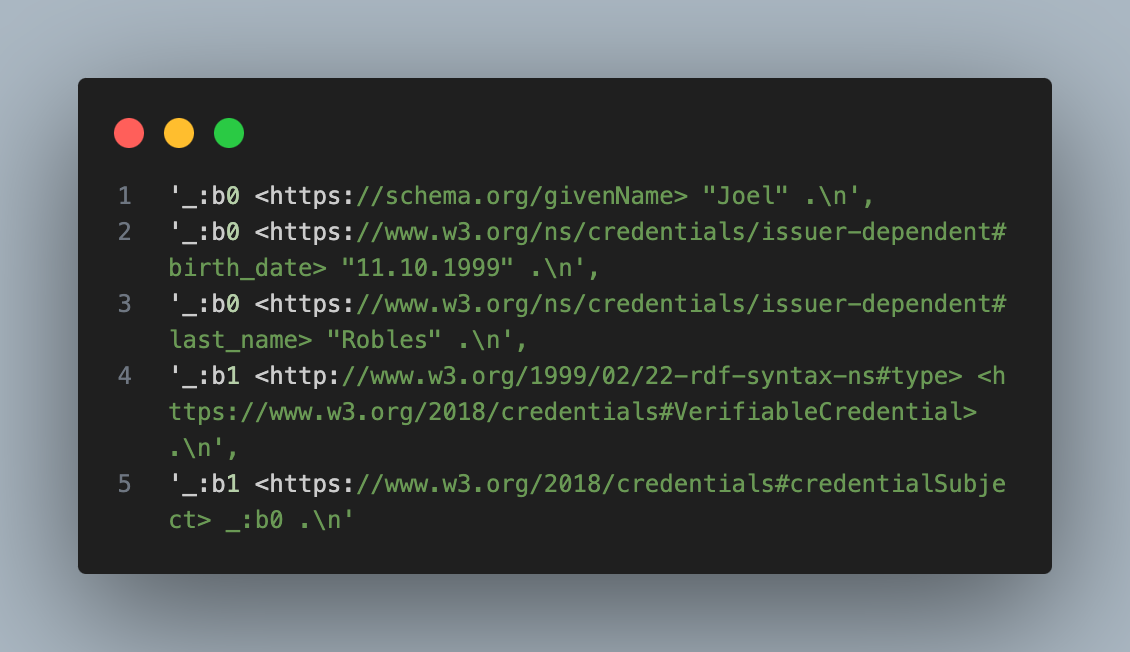
\includegraphics[width=70mm]{./img/VPcanon.png}
            \caption{Example Canonicalized VP}
        \end{figure}

    \end{columns}
\end{frame}

\section{Security Considerations}

\begin{frame}{Shuffling of statements}
    \begin{itemize}
        \item The verifier now gets a VP from the holder, which can be verified against the public key of the issuer
        \item Now let's assume that the holder gets a new version of the credential from the issues, where an attribute has been changed
        \item In a very specific case, the determinism of the RDF canonicalization algorithm can lead to data leakage
        \item That is why on each time this algorithm is used, the canonical statements must be shuffled using a has function
    \end{itemize}
\end{frame}

\end{document}